\documentclass{article}

% The authors should use one of these tracks.
% Before accepting by the NeurIPS conference, select one of the options below.
% 0. "default" for submission
% \usepackage{neurips_2025}
% the "default" option is equal to the "main" option, which is used for the Main Track with double-blind reviewing.
% 1. "main" option is used for the Main Track
\usepackage[main]{neurips_2025}
% 2. "position" option is used for the Position Paper Track
%  \usepackage[position]{neurips_2025}
% 3. "dandb" option is used for the Datasets & Benchmarks Track
 % \usepackage[dandb]{neurips_2025}
% 4. "creativeai" option is used for the Creative AI Track
%  \usepackage[creativeai]{neurips_2025}
% 5. "sglblindworkshop" option is used for the Workshop with single-blind reviewing
 % \usepackage[sglblindworkshop]{neurips_2025}
% 6. "dblblindworkshop" option is used for the Workshop with double-blind reviewing
%  \usepackage[dblblindworkshop]{neurips_2025}

% After being accepted, the authors should add "final" behind the track to compile a camera-ready version.
% 1. Main Track
 % \usepackage[main, final]{neurips_2025}
% 2. Position Paper Track
%  \usepackage[position, final]{neurips_2025}
% 3. Datasets & Benchmarks Track
 % \usepackage[dandb, final]{neurips_2025}
% 4. Creative AI Track
%  \usepackage[creativeai, final]{neurips_2025}
% 5. Workshop with single-blind reviewing
%  \usepackage[sglblindworkshop, final]{neurips_2025}
% 6. Workshop with double-blind reviewing
%  \usepackage[dblblindworkshop, final]{neurips_2025}
% Note. For the workshop paper template, both \title{} and \workshoptitle{} are required, with the former indicating the paper title shown in the title and the latter indicating the workshop title displayed in the footnote.
% For workshops (5., 6.), the authors should add the name of the workshop, "\workshoptitle" command is used to set the workshop title.
% \workshoptitle{WORKSHOP TITLE}

% "preprint" option is used for arXiv or other preprint submissions
 % \usepackage[preprint]{neurips_2025}

% to avoid loading the natbib package, add option nonatbib:
%    \usepackage[nonatbib]{neurips_2025}

\usepackage[utf8]{inputenc} % allow utf-8 input
\usepackage[T1]{fontenc}    % use 8-bit T1 fonts
\usepackage{hyperref}       % hyperlinks
\usepackage{url}            % simple URL typesetting
\usepackage{booktabs}       % professional-quality tables
\usepackage{amsfonts}       % blackboard math symbols
\usepackage{nicefrac}       % compact symbols for 1/2, etc.
\usepackage{microtype}      % microtypography
\usepackage{xcolor}         % colors

\usepackage{graphicx}
\usepackage{subcaption}
% Attempt to make hyperref and algorithmic work together better:
% \newcommand{\theHalgorithm}{\arabic{algorithm}}
\usepackage{tikz}
\usepackage{amsmath}
\usepackage{amssymb}
\usepackage{mathtools}
\usepackage{amsthm}
\usepackage{enumitem}

% Define theorem-like environments
\newtheorem{definition}{Definition}[section]

% if you need to pass options to natbib, use, e.g.:
%     \PassOptionsToPackage{numbers, compress}{natbib}
% before loading neurips_2025


% Note. For the workshop paper template, both \title{} and \workshoptitle{} are required, with the former indicating the paper title shown in the title and the latter indicating the workshop title displayed in the footnote. 
\title{Markovian Transformers for Informative Language Modeling}
\workshoptitle{Markovian Transformers for Informative Language Modeling}


% The \author macro works with any number of authors. There are two commands
% used to separate the names and addresses of multiple authors: \And and \AND.
%
% Using \And between authors leaves it to LaTeX to determine where to break the
% lines. Using \AND forces a line break at that point. So, if LaTeX puts 3 of 4
% authors names on the first line, and the last on the second line, try using
% \AND instead of \And before the third author name.


\author{%
  Scott Viteri\thanks{Corresponding author: sviteri@stanford.edu} \\
  Department of Computer Science\\
  Stanford University\\
  Stanford, CA, USA \\
  \And
  Max Lamparth \\
  Department of Computer Science\\
  Stanford University\\
  Stanford, CA, USA \\
  \And
  Peter Chatain \\
  Department of Computer Science\\
  Stanford University\\
  Stanford, CA, USA \\
  \And
  Clark Barrett \\
  Department of Computer Science\\
  Stanford University\\
  Stanford, CA, USA \\
}


\begin{document}


\maketitle


\begin{abstract}
  Chain-of-Thought (CoT) reasoning often fails to faithfully reflect a language model's underlying decision process. We address this by introducing a \emph{Markovian} language model framework that structurally enforces CoT text to be causally essential, factoring next-token prediction through an intermediate CoT and training it to predict future tokens independently of the original prompt. Within this framework, we apply an informativeness objective to ensure the CoT effectively supports predictions, achieving a 33.2\% absolute accuracy improvement on GSM8K with Llama 3.1 8B. Perturbation tests confirm stronger reliance on the CoT, while cross-model transfers indicate these reasoning traces generalize across interpreters. Our approach enhances both accuracy and interpretability, potentially extending CoT reasoning to arbitrarily long contexts and diverse tasks.
\end{abstract}


\section{Introduction}
\label{sec:intro}
The rapid advancement of language models (LMs) has led to impressive performance on complex cognitive tasks~\citep{NEURIPS2020_1457c0d6}. Yet it is often unclear \emph{why} an LM arrives at a particular conclusion~\citep{lamparth2023analyzing,burns2024discovering,gurnee2024language}, causing issues in high-stakes applications~\citep{Grabb2024.04.07.24305462,lamparth2024human,rivera2024escalation}. Traditional interpretability methods analyze hidden activations or attention patterns to extract ``explanations''~\citep{geiger2022inducing,geva2022transformer,meng2022locating,raukur2022toward,wang2022interpretability,lamparth2023analyzing,nanda2023progress}. Modern LMs, however, already generate coherent text: we might hope \emph{prompting} the model to articulate its reasoning (``Chain-of-Thought'' or CoT)~\citep{nye2022show,wei2022chain} would yield a faithful record of its thought process. 

Unfortunately, CoT explanations can be \emph{unfaithful}. For example, \citet{turpin2023language} show that spurious in-context biases often remain hidden in the CoT, and \citet{lanham2023measuring} find that altering CoT text may not affect the final answer. Such observations indicate that standard CoTs are not ``load-bearing.''

In this work, we take a \emph{pragmatic} approach to interpretability, focusing on \emph{informativeness} over full faithfulness. Rather than insisting the CoT mirrors the model's entire internal process, we require that \emph{the CoT alone suffices to produce the final answer}. In other words, if we remove the original prompt and rely only on the CoT, the model should still reach the correct output. This makes the CoT \emph{causally essential} and \emph{fragile}: changing it necessarily alters the prediction.

What distinguishes our approach is the clear distinction between the model \emph{relying on its CoT} versus generating \emph{more informative CoTs}. While traditional approaches train models to generate better-quality CoTs, they don't fundamentally change how the model uses them. Our Markovian framework, by contrast, forces the model to process information through the CoT bottleneck, making the CoT not just informative but \emph{causally load-bearing} for prediction.

For instance, Mistral-7B's CoT on arithmetic tasks changed dramatically after training. \textbf{Before training}, it simply listed all numbers and their (incorrect) sum (e.g., ``Sum = 76 + 90 + 92 + ... = 2314''). \textbf{After training}, it performed correct step-by-step calculations (e.g., ``calculate 6 + 89 = 95; Next, calculate 95 + 38 = 133...''), breaking the task into manageable steps that can be verified independently and enabling accurate answer prediction even when the original question is removed.

\paragraph{Recipient-Specific Compression.}
A key insight is that an \emph{informative} CoT can also serve as a \emph{recipient-specific compression} of the model's hidden knowledge: it distills the essential reasoning into text that another recipient (e.g.\ a different model or a human) can use to predict the same outcome. Our experiments confirm that the learned CoTs generalize across interpreters, suggesting that these textual explanations genuinely encode transferable problem-solving steps rather than model-specific quirks (Section~\ref{subsec:interp}).

\paragraph{Contributions.}
\begin{enumerate}
    \item We introduce a Markovian language model framework that structurally enforces Chain-of-Thought (CoT) generation to be causally essential, ensuring reliance on the CoT for predictions.
    \item We apply this framework to arithmetic problems (Mistral 7B) and the GSM8K dataset~\citep{cobbe2021gsm8k} (Llama 3.1 8B), observing a 33.2\% absolute improvement on GSM8K.
    \item We show that perturbing the CoT consistently degrades prediction accuracy, verifying \emph{fragility} and causal relevance.
    \item We demonstrate cross-model transfer: CoTs trained on one model remain informative for other models. This underscores the CoT's \emph{recipient-specific} interpretability and suggests it captures a shared reasoning strategy.
\end{enumerate}

Section~\ref{sec:related_work} reviews related work, Section~\ref{sec:MLM} details our Markovian framework, and Section~\ref{sec:method} describes the RL training. Section~\ref{sec:experiments} presents empirical results, and Section~\ref{sec:disc} discusses limitations and future directions.


\begin{figure*}[t!]
  \centering
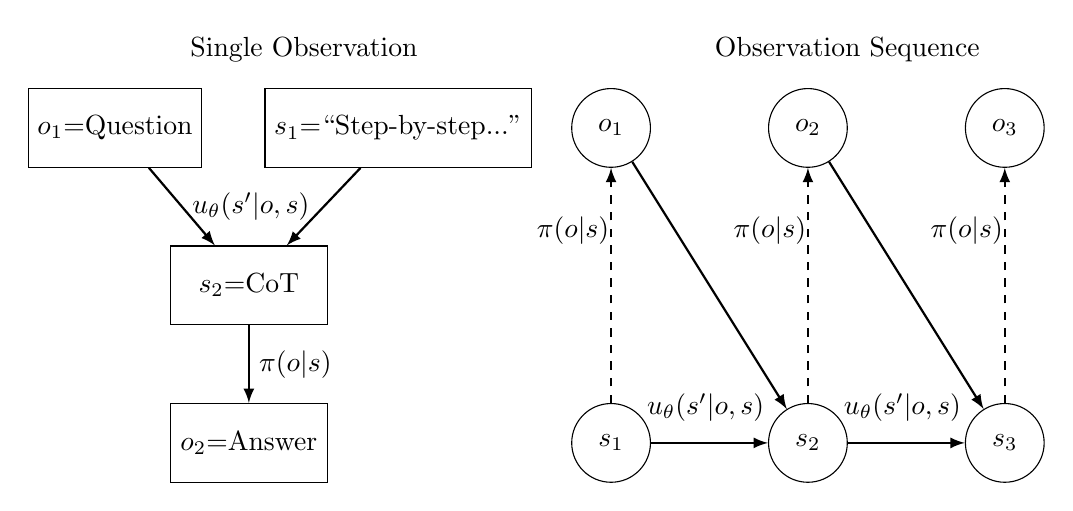
\begin{tikzpicture}[
    node distance=2cm,
    box/.style={rectangle, draw, minimum width=2cm, minimum height=1cm},
    circlebox/.style={circle, draw, minimum size=1cm},
    arrow/.style={->, thick},
    >=latex
]

% Left side: Single timestep
\node[box] (Q) at (-4.3,2) {$o_1$=Question};
\node[box] (S) at (-0.7,2) {$s_1$=``Step-by-step...''};
\node[box] (CoT) at (-2.6,0) {$s_2$=CoT};
\node[box] (A) at (-2.6,-2) {$o_2$=Answer};

\draw[arrow] (Q) -- node[right] {$u_\theta(s'|o,s)$} (CoT);
\draw[arrow] (S) -- (CoT);
\draw[arrow] (CoT) -- node[right] {$\pi(o|s)$} (A);

% Right side: Causal structure
% Observations
\node[circlebox] (o1) at (2,2) {$o_1$};
\node[circlebox] (o2) at (4.5,2) {$o_2$};
\node[circlebox] (o3) at (7,2) {$o_3$};

% States
\node[circlebox] (s1) at (2,-2) {$s_1$};
\node[circlebox] (s2) at (4.5,-2) {$s_2$};
\node[circlebox] (s3) at (7,-2) {$s_3$};

% Connections
\draw[arrow] (o1) to (s2);
\draw[arrow] (s1) to (s2);
\node[above] at (3.2,-1.85) {$u_\theta(s'|o,s)$};

\draw[arrow] (o2) to (s3);
\draw[arrow] (s2) to (s3);
\node[above] at (5.7,-1.85) {$u_\theta(s'|o,s)$};

% π(o|s) connections
\draw[arrow, dashed] (s1) to (o1);
\node[left] at (2.1,0.7) {$\pi(o|s)$};

\draw[arrow, dashed] (s2) to (o2);
\node[left] at (4.6,0.7) {$\pi(o|s)$};

\draw[arrow, dashed] (s3) to (o3);
\node[left] at (7.1,0.7) {$\pi(o|s)$};

% Labels
\node at (-1.9,3) {Single Observation};
\node at (5,3) {Observation Sequence};

\end{tikzpicture}
\caption{Refined illustration of the training method. Left: Single time-step process from Question to CoT to Answer. Right: Causal structure showing the generation of states from observations and previous states using the state update function $u_\theta(s'|o,s)$, and the prediction of observations from states using the policy $\pi(o|s)$. Observations are generated by the causal data distribution. In experiments, both $u_\theta$ and $\pi$ are Mistral 7B Instruct V0.2 or Llama 3.1 8B Instruct, but only the weights of $u_\theta$ are updated during training. The state update $u_\theta$ also involves concatenating the observation and state letting Mistral generate the next state's worth of tokens.}
\label{fig:training-method-causal-final}
\end{figure*}

\begin{figure*}
  \centering
    \includegraphics[width=\textwidth]{Figures/cot_performance_comparison.png}
    \caption{The log probability $\ln \pi(\text{ans} \mid \text{CoT})$ of the answer $ans$ given a $\text{CoT}$, where the $\text{CoT}$ is sampled from the trained weights $\text{CoT} \sim u_\theta(\text{CoT} \mid q, \text{CoT}_{\text{init}})$ and $\text{CoT}'$ is sampled from the unmodified weights $\text{CoT}' \sim u(\text{CoT} \mid q, \text{CoT}_{\text{init}})$. We train to produce CoTs which are sufficient to predict the correct answer even without the original question, enforcing a text bottleneck in the language model's information flow, forcing the CoT to be causally load-bearing to production of the answer. This plot specifically depicts the training of Mistral 7B Instruct V0.2 on fifteen-term addition problems and their solutions. Because of high variance, we plot the point-wise maximum \emph{over four runs} for each training technique.}
    \label{fig:loss}
\end{figure*}

\section{Related Work}
\label{sec:related_work}

Prior work shows that CoT prompting can boost performance on reasoning tasks \citep{wei2022chain, nye2022show}.
Whereas typical CoT prompting methods do not alter a pre-trained model's parameters, some prior approaches do fine-tune the model for CoT generation \citep{eric_star2022, zelikman2024quietstar, deepseekai2025}. Our work differs by removing the original question or passage from the answer-prediction context, which enforces a stronger causal reliance on the CoT.

Regarding faithfulness vs. interpretability, some authors discuss how a CoT may fail to reflect the true reason the LM arrived at its answer \citep{lanham2023measuring, turpin2023language}, since small changes in the CoT do not necessarily change the final prediction. \citet{zhou2023understanding} analyze CoT through an information-theoretic lens, finding that CoT can serve as a communication channel between different parts of a model. We build on these insights by \emph{training} the model to rely on this channel exclusively.

Architecturally, our Markovian LM shares structural similarities with state space models like RNNs \citep{rumelhart1986learning}, S4 \citep{gu2022efficientlymodelinglongsequences}, and Mamba \citep{gu2024mamba}, though with a key difference: MLMs have probabilistic state transitions to model token sampling, which necessitates gradient estimation methods such as policy gradient \citep{policy_gradient} rather than direct backpropagation. This probabilistic structure also resembles Kalman filters \citep{proto_pomdp1965}, Deep Variational Bayes Filters \citep{karl2017deepvariationalbayesfilters}, Deep Kalman Filters \citep{krishnan2015deepkalmanfilters}, and Variational Recurrent Neural Networks (VRNN) \citep{DBLP:journals/corr/ChungKDGCB15}, though we use categorical rather than Gaussian distributions for interpretable text generation. Other fine-tuned reasoning models mentioned above (R1, STaR, and QuietSTaR) have similar structure but allow seeing the full context before generating state/reasoning tokens, whereas our approach enforces a strict information bottleneck through the state.

\citet{lyu2023faithful} also consider restricting the model's ability to see the original input while generating the final answer. Their approach, however, involves rewriting the question in a structured formal language or code that is then executed. Our approach uses natural language for the reasoning state to preserve interpretability across diverse tasks.

\section{Markovian Language Models and Informativeness}
\label{sec:MLM}

Here we provide our formalism for Markovian Language Models (MLMs) and define \emph{informativeness}, which we use as a training objective within our novel structural framework.

\subsection{Markovian Language Models (MLM)}

A traditional LM can attend to the entire context when predicting the next token. This makes it possible for an LM to disregard the CoT or only partially rely on it. We impose a stricter, \emph{Markovian} structure\footnote{This structure can be viewed as a stochastic variant of a Moore machine where both the transition function ($u$) and output function ($\pi$) are probabilistic, and the input and output alphabets are identical ($O$). Alternatively, an MLM can be formalized as an F-coalgebra where F(S) = P(O) $\times$ P(S)$^O$, with P representing probability distributions.}:
\begin{definition}[Markovian LM]
A Markovian Language Model is a tuple $M=(\mathcal{O}, \mathcal{S}, \pi, u, s_1)$, where
\begin{itemize}
\item $\mathcal{O}$ is a set of observations (e.g., questions and answers in a QA task),
\item $\mathcal{S}$ is a set of states (e.g., CoT reasoning text),
\item $\pi: \mathcal{S}\rightarrow \Delta(\mathcal{O})$ is a policy that predicts the next observation from the state alone,
\item $u: \mathcal{O}\times\mathcal{S}\rightarrow \Delta(\mathcal{S})$ is a state update function (produces CoT from question and initial prompt),
\item $s_1\in \mathcal{S}$ is an initial state (starting CoT prompt).
\end{itemize}
\end{definition}

For example, in a math reasoning task, $o_1 \in \mathcal{O}$ might be a question, $s_1 \in \mathcal{S}$ is an initial CoT prompt like ``Let's solve this step-by-step:'', $s_2 \in \mathcal{S}$ is the generated reasoning chain, and $o_2 \in \mathcal{O}$ is the answer. The key idea is that $\pi$ can only see the CoT state $s_2$ when predicting $o_2$, forcing the CoT to contain all needed information. Intuitively, $\pi$ is the \emph{frozen} next-token predictor, and $u$ is the model's \emph{trainable} component that chooses how to produce the CoT from the latest observation and prior state. In our experiments, $\pi$ and $u$ share the same underlying transformer but we freeze the weights for $\pi$ while fine-tuning those used by $u$. 

\subsection{Data-Generating Distribution and Reward}

Let $P$ be the distribution over observations $x_1, x_2, \dots, x_T \in \mathcal{O}$. A trajectory $\tau$ is generated by:
\[
s_{t+1}\sim u(s_t, x_t), \quad x_{t+1}\sim P(x_{t+1}\mid x_{\le t}),
\]
with $s_1$ a fixed initial prompt. We define the \emph{reward} for a trajectory $\tau$ as:
\[
R(\tau)=\sum_{t=1}^T \left[\ln \pi(x_t\mid s_t)-\ln \pi(x_t\mid s'_t)\right],
\]
where $s'_t$ is generated by a \emph{baseline} update function $u'$, e.g., the \emph{untrained} model. In words, $R(\tau)$ measures how much more likely the correct observation $x_t$ is under the trained state $s_t$ compared to the baseline state $s'_t$.

\subsection{Informativeness Objective}

Conceptually, we aim to ensure that the CoT state serves as a critical bottleneck for information flow, making it causally essential for predictions. Formalizing this within our Markovian framework, we define:
\[
  J(\theta)=\mathbb{E}_{\tau \sim P,u_\theta,u'}\left[R(\tau)\right],
\]
where $\theta$ parameterizes $u_\theta$. Maximizing $J(\theta)$ ensures that the update function $u_\theta$ produces states $s_t$ that are \emph{informative} about future observations (relative to the baseline $u'$), thereby enforcing the CoT's role as a load-bearing component. We optimize $J(\theta)$ with policy gradient or PPO, sampling observations from $P$ and states from $u_\theta$ and $u'$.

\section{Methods}
\label{sec:method}

\subsection{Implementation as Question-Answer Pairs}
In many tasks like math problem solving, we have $T=2$ observations (question and answer) and implement the abstract MLM with a fixed maximum length for the CoT state. Let $\mathcal{V}$ be a token vocabulary. We set $\mathcal{O} = \mathcal{V}^N$ and $\mathcal{S} = \mathcal{V}^K$ for some $N, K \in \mathbb{N}$, where $K$ is the maximum tokens in the CoT. Note that while we limit the state to a maximum of $K$ tokens for implementation, we do not enforce fixed-length observations. 

Our conceptual arguments rely on $K < N$, as otherwise the model could simply write the predicted observation into the state. We satisfy this in our Wikipedia experiments (Sec~\ref{subsec:wikipedia}), and for other experiments we find empirically that the model does not learn this undesirable behavior due to the difficulty of predicting the answer directly without any CoT.

In this setting, we denote our states as $s_1 = \text{CoT}_{\text{init}}$ and $s_2 = \text{CoT}$, where $\text{CoT}_{\text{init}}$ is a task-specific prompt\footnote{The exact prompt template varies by task type, with each template specifying the task objective, allowed $\text{CoT}$ length, and an invitation to reason strategically. Full templates are provided in Sec~\ref{subsec:stability}.}. With pre-trained LM $\mathcal{L}$, we can implement our update function $u$ and policy $\pi$ using:
\begin{align}
\ln u\bigl(s_2 = \text{CoT} \,\mid\, q, s_1 = \text{CoT}_{\text{init}}\bigr) &= 
\sum_{i=1}^{K}
    \ln \mathcal{L}\!\Bigl(\text{concat}\bigl(q,\,
    \text{CoT}_{\text{init}},\, \text{CoT}_{<i}\bigr)\Bigr)\bigl[\text{CoT}_i\bigr], \\[1em]
\ln \pi(\text{ans} \mid \text{CoT}) &=  \sum_{i=1}^{N} \ln \mathcal{L}(\text{concat}(\text{CoT}, \text{ans}_{<i})) [\text{ans}_i].
\end{align}

Crucially, we do \emph{not} allow the answer generation to attend back to the question $q$ directly; the question is replaced by the $\text{CoT}$. For each question $q$, we generate the baseline state $s'_2$ (which we denote as $\text{CoT}'$ in this setting) by prompting the unmodified pre-trained model with $q$ plus an initial instruction (e.g., 'Think step-by-step...'), and recording its raw output.

Our reward is:
\[
R = \ln \pi(\text{ans} \mid \text{CoT}) \;-\; \ln \pi(\text{ans} \mid \text{CoT}').
\]

\subsection{Reinforcement Learning Objectives}
\label{subsec:rl_objectives}
Having defined the reward in terms of CoT informativeness, we explore three RL techniques to optimize $u_\theta$ toward producing high-reward CoTs. All three rely on sampling $\text{CoT}$ and $\text{CoT'}$ for a given question $q$, then comparing their contributions to the final answer likelihood. 

\subsubsection{Threshold-based Expert Iteration (TEI)}
\label{subsubsec:tei}
Threshold-based Expert Iteration consists of the following steps:
\begin{enumerate}
    \item Sample $\text{CoT}$ from the trained policy $u_\theta$ and a baseline $\text{CoT'}$ from $u'$ for the same question $q$.
    \item Estimate informativeness $I(\text{ans}, \text{CoT}, \text{CoT'}) \;=\; \pi(\text{ans}\mid \text{CoT}) \;-\; \pi(\text{ans}\mid \text{CoT'})$.
    \item If $I$ is at least one standard deviation above the historical average:
\begin{itemize}
            \item Compute $\nabla_\theta \ln u_\theta(\text{CoT} \mid q, \text{CoT}_{\text{init}})$.
            \item Perform gradient ascent on $\theta$.
\end{itemize}
\end{enumerate}
\noindent
\textbf{Limitation:} TEI discards CoTs that yield moderate but still valuable rewards, potentially slowing learning.

\subsubsection{Policy Gradient (PG)}
\label{subsubsec:pg}
Policy Gradient with thresholding extends TEI by weighing updates by $I$:
\begin{enumerate}
    \item Sample $\text{CoT}$ and a baseline $\text{CoT'}$ for each question $q$.
    \item Compute $I = \pi(\text{ans}\mid \text{CoT}) - \pi(\text{ans}\mid \text{CoT'})$.
    \item If $I$ is at least one standard deviation above its historical mean:
\begin{itemize}
            \item Calculate $\nabla_\theta \ln u_\theta(\text{CoT} \mid q, \text{CoT}_{\text{init}})$.
            \item Scale this gradient by $I$ and ascend.
\end{itemize} 
\end{enumerate}
\noindent
\textbf{Advantage:} Uses more of the reward signal, accelerating learning. \\
\textbf{Disadvantage:} Potentially more instability, especially if $I$ is large or negative.

\subsubsection{Proximal Policy Optimization (PPO)}
\label{subsubsec:ppo}
PPO clips probability ratios to stabilize large policy updates:
\begin{enumerate}
    \item For a sampled CoT $\text{CoT}$, compute the ratio $r = \frac{u_\theta(\text{CoT}\mid q,\text{CoT}_{\text{init}})}{u'(\text{CoT}\mid q,\text{CoT}_{\text{init}})}$.
    \item Let $I = \pi(\text{ans}\mid \text{CoT}) - \pi(\text{ans}\mid \text{CoT'})$ be the informativeness reward.
    \item Define the clipped objective:
    \[
    \text{obj} = \min\!\Bigl(r \cdot I, \;\text{clip}(r,1-\epsilon,1+\epsilon)\cdot I\Bigr), 
     \text{where } \epsilon=0.2.
    \]
    \item Ascend on $\nabla_\theta \text{obj}$.
\end{enumerate}
\textbf{Key Idea:} PPO discourages the new CoT distribution $u_\theta$ from diverging too sharply from $u'$, thus trading off exploration and stability.  


\subsection{Training Stability and Implementation Details}
\label{subsec:stability}
Fine-tuning a pre-trained language model with a strong linguistic prior requires careful consideration to avoid irrecoverable weight updates that could push the model out of the language modeling loss basin. In addition to the PPO-clip objective mentioned in Sec.~\ref{subsubsec:ppo}, we implemented several techniques to enhance training stability across different objective functions:

\begin{enumerate}
    \item \textbf{Low-Rank Adaptation (LoRA) \citep{hu2022lora}:} 
    \begin{itemize}
        \item Freeze all weights except for small-rank LoRA adapters.
        \item Use rank 8 with $\alpha = 16$.
    \end{itemize}

    \item \textbf{Gradient Clipping:} 
    \begin{itemize}
        \item If the $\ell_2$ norm of the gradient exceeds $1.0$, rescale it to norm $1.0$.
    \end{itemize}

    \item \textbf{Gradient Accumulation (Arithmetic Only):} 
    \begin{itemize}
        \item For arithmetic tasks, set batch size to 6 (to fit on one H100 GPU).
        \item Accumulate gradients for 8 steps before updating weights.
    \end{itemize}

    \item \textbf{Average Reward Baseline:} 
    \begin{itemize}
        \item For PPO (and PG variants), we subtract a running average of past rewards from the current reward to stabilize updates.
        \item This replaces a learned value function with a simpler baseline, reducing hyperparameter tuning.
    \end{itemize}

    \item \textbf{Initial CoT Prompt Design:} 
    \begin{itemize}
        \item Choose $\text{CoT}_{\text{init}}$ to guide the model toward meaningful reasoning. 
        \item For arithmetic: 
        \begin{quote}
            \small
            ``You will be given an arithmetic problem, which you have [CoT length] tokens to work through step-by-step. Question:''
        \end{quote}
        \item For GSM8K:
        \begin{quote}
            \small
            ``You will be given a reasoning problem, which you have [CoT length] tokens to work through step-by-step. Question:''
        \end{quote}
        \item For Wikipedia:
        \begin{quote}
            \small
            ``You will need to predict the next [target length] tokens which follow the provided passage. You can write [CoT length] thinking tokens which will be your sole context for prediction. Feel free to be creative in your thinking strategy! Opening text:''
        \end{quote}
    \end{itemize}
\end{enumerate}

These measures greatly reduce the risk of catastrophic updates and keep the model's training on track.



\section{Experiments}
\label{sec:experiments}
\begin{figure*}
    \centering
    \includegraphics[width=\textwidth]{Figures/llama_combined_metrics_gsm8k.png}
    \caption{GSM8K performance metrics over three separate training runs of Llama-3.1-8B-Instruct. The left plot shows the log probability that an untrained Llama assigns to the correct answer given the trained CoT --- $\ln \pi(\text{ans}|\text{CoT})$, and the right plot shows the proportion of CoTs in a batch which contain the answer verbatim. We use a smoothing window of size 100, explaining the multiplicity of possible y-values for ``Contains Answer''.}
    \label{fig:gsm8k_performance}
\end{figure*}

\subsection{Multi-step Addition}
\label{subsec:solving}
We generate random addition problems, where each problem consists of fifteen terms and each term is a uniform random natural number less than 100. We fine-tune Mistral 7B Instruct V0.2 to produce CoT tokens such that a frozen copy of the pre-trained language model can predict the correct answer given that CoT, for each training technique in Sec~\ref{sec:method}. We plot the mean negative log likelihood over the answer tokens as a function of training batch in Fig.~\ref{fig:loss}. Note that this is both training and testing loss, since we are always generating fresh arithmetic problems. PPO, our preferred training method for arithmetic, can mention the correct answer in up to 90\% of CoTs and achieve an average natural log probability of around -0.7. 

Since the Mistral tokenizer allocates a separate token for each digit, a natural log probability of -0.7 corresponds to about 50\% probability ($e^{-0.7} \approx 0.4966$) per token. The seeming contradiction between 90\% verbatim answer likelihood and 50\% per-digit uncertainty stems from the predictor's format uncertainty—it distributes probability across the entire vocabulary when deciding what follows "Answer:", as we only train CoT production $u_\theta(s'|o,s)$, not the predictor $\pi(o|s)$.

\subsection{GSM8K}
\label{subsec:gsm8k}
To test our method on more complex reasoning tasks, we train Llama-3.1-8B-Instruct on GSM8K using policy gradient with expert iteration (threshold 2.2 standard deviations) and a KL penalty (0.1). We produce up to 150 CoT tokens and estimate the value function with an exponentially decaying average of previous rewards (decay 0.9).

In Figure~\ref{fig:gsm8k_performance}, we show CoT informativeness (left) and proportion of CoTs containing verbatim answers (right). We observe a dramatic increase in exact-match accuracy from 35.94\% baseline to 69.14\% in our best run—a 33.2\% absolute improvement. The other runs (58.23\% and 62.85\%) confirm consistent effectiveness on mathematical reasoning.

\subsection{Wikipedia}
\label{subsec:wikipedia}

We also explored applying our approach to general language modeling using Wikipedia text. For each article, we condition on the first 200 tokens and task the model with predicting the following 100 tokens, allowing 50 tokens of CoT to aid prediction. Training parameters match those used in GSM8K (Sec~\ref{subsec:gsm8k}).

Results showed modest improvements in next-token prediction accuracy from 8.2\% to 10.5\% (supplement). This should be contextualized against pre-trained Llama's typical 16.9\% accuracy (over 10,000 articles) on the 200\textsuperscript{th} to 300\textsuperscript{th} tokens without context. The lower baseline (8.2\%) likely stems from our setup with CoT followed by `` Answer: '' before prediction. Despite this, key findings about CoT reliability remain evident: as Fig~\ref{fig:perturbation} shows, perturbing trained CoTs degrades accuracy more than perturbing baseline CoTs, indicating genuine CoT reliance.
\textbf{See supplement for examples of CoT changes after training.}

\begin{figure*}[ht]
  \centering
  \includegraphics[width=\textwidth]{Figures/combined_perturbation_plot_comparison_question_centered.png}
  \caption{Impact of perturbations on CoT effectiveness with/without the original question. Three perturbation types shown: character deletion, front truncation, and random replacement. Higher values indicate stronger reliance on CoT when the question is absent, showing causal dependence rather than just improved accuracy.}
  \label{fig:perturbation}
\end{figure*}


\subsection{Measuring Fragility of CoT}\label{subsec:fragile}

Expanding upon \citet{lanham2023measuring}, we gauge model dependence on CoT tokens using three perturbations: character deletion, front truncation, and random character replacement.
    
To isolate genuine fragility from improved accuracy, we use a question-centered metric that compares perturbation effects with and without the original question:
\begin{align}
m_2 &= [\ln P(\text{ans}|\text{CoT}) - \ln P(\text{ans}|\text{perturb}(\text{CoT}))] \nonumber\\
&- [\ln P(\text{ans}|q, \text{CoT}) - \ln P(\text{ans}|q, \text{perturb}(\text{CoT}))]
\end{align}

This metric directly measures how much the model relies on the CoT when the question is absent versus present. As shown in Fig.~\ref{fig:perturbation}, this difference increases significantly during training, confirming that our CoTs become genuinely more load-bearing rather than simply more accurate.

\subsection{Interpretability of CoT Generations}
\label{subsec:interp}

\begin{figure*}[ht]
  \centering
  \includegraphics[width=.9\textwidth]{Figures/wiki_multi_critic_comparison.png}
  \caption{Cross-model evaluation showing Llama-3.1-8B-Instruct's evaluation of Mistral's CoT quality throughout training on Wikipedia text prediction. The correlation between improvements in both models' evaluations suggests the learned reasoning patterns generalize across architectures rather than being model-specific artifacts. Each plot is averaged across 6 independent training runs.}
  \label{fig:cross_eval}
\end{figure*}

To probe how well the reasoning generalizes, we plot the informativeness of Llama's trained CoTs with respect to various other LMs on the Wikipedia dataset in Fig.~\ref{fig:cross_eval}. In both plots the normalized log probabilities increase simultaneously, demonstrating that Llama is learning to produce generic CoTs which do not over-fit to the peculiarities of a Llama answer-predictor. 

This cross-model transferability addresses a key question: ``interpretable to whom?'' We test across three distinct model families (Phi \citep{abdin2024phi3technicalreporthighly}, Mistral, and GPT2), including GPT2, a significantly smaller model that shouldn't be able to decode sophisticated steganography. The fact that trained CoTs transfer effectively across this diverse set confirms they contain generalizable reasoning patterns rather than model-specific artifacts.

\section{Discussion and Limitations}
\label{sec:disc}

Experiments across arithmetic, GSM8K, and Wikipedia show that it is possible to learn informative and interpretable CoT reasoning via RL on an LM using Markovian training.

However, our interpretability technique is currently only verified in myopic question-answer datasets, as opposed to multi-turn trajectories where trained CoTs might provide a lens into longer-term future behavior. In principle, the Markovian design naturally extends to multi-turn or multi-step settings by treating the CoT as recurrent state; we have not explored such tasks here for scope reasons.

Moreover, we have only evaluated interpretability by measuring \emph{model}-centric proxies (like CoT fragility and cross-model transfer). A more direct human evaluation would have people read the generated CoTs and attempt to predict the final answer, giving an explicit measure of whether these CoTs are genuinely human-interpretable. Such a setup could be incorporated into the training objective, where human correctness in predicting the answer provides an additional signal for optimizing CoT generation.

Markovian training is language modeling with an intermediate memory-producing action, similar to R1 recurrence and ``thinking'' models. This approach blurs the line between RL and unsupervised learning, though its expensive serial token generation requires justification through gains in interpretability or perplexity.

Our findings indicate that Markovian training yields substantial gains in CoT fragility (Sec~\ref{subsec:fragile}) and cross-model transfer (Sec~\ref{subsec:interp}), suggesting practical opportunities for improved interpretability. While human studies could further validate interpretability, we rely on cross-model transfer as a proxy and leave comprehensive trials to future work.

\paragraph{Future Work.}
Although we focus on single question–answer pairs, the Markovian framework extends to multi-turn dialogue. After each user message $o_t$, we produce the next CoT $s_{t+1}$ via $u_\theta(s_{t+1}\mid s_t,o_t)$, then generate the system's reply from that CoT alone. This process treats the CoT as a recurrent state, which could scale to conversation rounds.



\bibliography{neurips_2025}
\bibliographystyle{plainnat}


\newpage
\section*{NeurIPS Paper Checklist}

\begin{enumerate}

\item {\bf Claims}
    \item[] Question: Do the main claims made in the abstract and introduction accurately reflect the paper's contributions and scope?
    \item[] Answer: \answerYes{} % Replace by \answerYes{}, \answerNo{}, or \answerNA{}.
    \item[] Justification: The abstract and introduction clearly state our contributions: (1) a Markovian training procedure that makes CoT text causally essential, (2) experimental results showing substantial accuracy improvements, (3) evidence of CoT fragility through perturbation tests, and (4) demonstration of cross-model transferability. These claims are directly supported by our methodology and experiments in Sections 3-5. 
    \item[] Guidelines:
    \begin{itemize}
        \item The answer NA means that the abstract and introduction do not include the claims made in the paper.
        \item The abstract and/or introduction should clearly state the claims made, including the contributions made in the paper and important assumptions and limitations. A No or NA answer to this question will not be perceived well by the reviewers. 
        \item The claims made should match theoretical and experimental results, and reflect how much the results can be expected to generalize to other settings. 
        \item It is fine to include aspirational goals as motivation as long as it is clear that these goals are not attained by the paper. 
    \end{itemize}

\item {\bf Limitations}
    \item[] Question: Does the paper discuss the limitations of the work performed by the authors?
    \item[] Answer: \answerYes{} % Replace by \answerYes{}, \answerNo{}, or \answerNA{}.
    \item[] Justification: Section 5 (Discussion and Limitations) thoroughly addresses the limitations of our approach. We acknowledge that our interpretability technique has only been verified on question-answer datasets rather than multi-turn trajectories, that we used model-centric proxies for interpretability rather than human evaluations, and that our Markovian training introduces computational costs due to serial token generation steps. We also discuss how these limitations affect the generalizability of our results and potential future extensions.
    \item[] Guidelines:
    \begin{itemize}
        \item The answer NA means that the paper has no limitation while the answer No means that the paper has limitations, but those are not discussed in the paper. 
        \item The authors are encouraged to create a separate "Limitations" section in their paper.
        \item The paper should point out any strong assumptions and how robust the results are to violations of these assumptions (e.g., independence assumptions, noiseless settings, model well-specification, asymptotic approximations only holding locally). The authors should reflect on how these assumptions might be violated in practice and what the implications would be.
        \item The authors should reflect on the scope of the claims made, e.g., if the approach was only tested on a few datasets or with a few runs. In general, empirical results often depend on implicit assumptions, which should be articulated.
        \item The authors should reflect on the factors that influence the performance of the approach. For example, a facial recognition algorithm may perform poorly when image resolution is low or images are taken in low lighting. Or a speech-to-text system might not be used reliably to provide closed captions for online lectures because it fails to handle technical jargon.
        \item The authors should discuss the computational efficiency of the proposed algorithms and how they scale with dataset size.
        \item If applicable, the authors should discuss possible limitations of their approach to address problems of privacy and fairness.
        \item While the authors might fear that complete honesty about limitations might be used by reviewers as grounds for rejection, a worse outcome might be that reviewers discover limitations that aren't acknowledged in the paper. The authors should use their best judgment and recognize that individual actions in favor of transparency play an important role in developing norms that preserve the integrity of the community. Reviewers will be specifically instructed to not penalize honesty concerning limitations.
    \end{itemize}

\item {\bf Theory assumptions and proofs}
    \item[] Question: For each theoretical result, does the paper provide the full set of assumptions and a complete (and correct) proof?
    \item[] Answer: \answerNA{} % Replace by \answerYes{}, \answerNo{}, or \answerNA{}.
    \item[] Justification: Our paper focuses on an empirical approach to Markovian language models and presents experimental results rather than formal theoretical results requiring proofs. While we provide a definition of Markovian LMs and an informativeness objective in Section 3, these serve as a framework for our methodology rather than theoretical results that would require formal proofs.
    \item[] Guidelines:
    \begin{itemize}
        \item The answer NA means that the paper does not include theoretical results. 
        \item All the theorems, formulas, and proofs in the paper should be numbered and cross-referenced.
        \item All assumptions should be clearly stated or referenced in the statement of any theorems.
        \item The proofs can either appear in the main paper or the supplemental material, but if they appear in the supplemental material, the authors are encouraged to provide a short proof sketch to provide intuition. 
        \item Inversely, any informal proof provided in the core of the paper should be complemented by formal proofs provided in appendix or supplemental material.
        \item Theorems and Lemmas that the proof relies upon should be properly referenced. 
    \end{itemize}

    \item {\bf Experimental result reproducibility}
    \item[] Question: Does the paper fully disclose all the information needed to reproduce the main experimental results of the paper to the extent that it affects the main claims and/or conclusions of the paper (regardless of whether the code and data are provided or not)?
    \item[] Answer: \answerYes{} % Replace by \answerYes{}, \answerNo{}, or \answerNA{}.
    \item[] Justification: Our Reproducibility Statement (in the appendix) provides comprehensive details for reproducing our results. We specify all code components (\texttt{src/train.py}, \texttt{src/perturbation\_analysis.py}, \texttt{src/evaluate\_cross\_model.py}), datasets used (GSM8K, HuggingFace Wikipedia), model architectures (Llama 3.1 8B, Mistral 7B, etc.), and implementation details needed to recreate our experiments. Section 3.3 further details our training methodologies, and we specify hyperparameters throughout the paper. Additionally, we'll release our code repository with documentation for reproducing all experimental results.
    \item[] Guidelines:
    \begin{itemize}
        \item The answer NA means that the paper does not include experiments.
        \item If the paper includes experiments, a No answer to this question will not be perceived well by the reviewers: Making the paper reproducible is important, regardless of whether the code and data are provided or not.
        \item If the contribution is a dataset and/or model, the authors should describe the steps taken to make their results reproducible or verifiable. 
        \item Depending on the contribution, reproducibility can be accomplished in various ways. For example, if the contribution is a novel architecture, describing the architecture fully might suffice, or if the contribution is a specific model and empirical evaluation, it may be necessary to either make it possible for others to replicate the model with the same dataset, or provide access to the model. In general. releasing code and data is often one good way to accomplish this, but reproducibility can also be provided via detailed instructions for how to replicate the results, access to a hosted model (e.g., in the case of a large language model), releasing of a model checkpoint, or other means that are appropriate to the research performed.
        \item While NeurIPS does not require releasing code, the conference does require all submissions to provide some reasonable avenue for reproducibility, which may depend on the nature of the contribution. For example
        \begin{enumerate}
            \item If the contribution is primarily a new algorithm, the paper should make it clear how to reproduce that algorithm.
            \item If the contribution is primarily a new model architecture, the paper should describe the architecture clearly and fully.
            \item If the contribution is a new model (e.g., a large language model), then there should either be a way to access this model for reproducing the results or a way to reproduce the model (e.g., with an open-source dataset or instructions for how to construct the dataset).
            \item We recognize that reproducibility may be tricky in some cases, in which case authors are welcome to describe the particular way they provide for reproducibility. In the case of closed-source models, it may be that access to the model is limited in some way (e.g., to registered users), but it should be possible for other researchers to have some path to reproducing or verifying the results.
        \end{enumerate}
    \end{itemize}


\item {\bf Open access to data and code}
    \item[] Question: Does the paper provide open access to the data and code, with sufficient instructions to faithfully reproduce the main experimental results, as described in supplemental material?
    \item[] Answer: \answerYes{} % Replace by \answerYes{}, \answerNo{}, or \answerNA{}.
    \item[] Justification: We will publicly release our full codebase, including all training and evaluation scripts mentioned in our Reproducibility Statement. Our experiments use publicly available datasets (GSM8K and HuggingFace Wikipedia) and models (Llama 3.1 8B Instruct, Mistral 7B Inst V0.2, Phi 3.5 Mini-Instruct, GPT2). Our code repository includes detailed instructions in the README for environment setup, data preparation, and experiment execution. The \texttt{results/Official} directory contains plots, training logs, and evaluation logs to enable comparison with future implementations.
    \item[] Guidelines:
    \begin{itemize}
        \item The answer NA means that paper does not include experiments requiring code.
        \item Please see the NeurIPS code and data submission guidelines (\url{https://nips.cc/public/guides/CodeSubmissionPolicy}) for more details.
        \item While we encourage the release of code and data, we understand that this might not be possible, so "No" is an acceptable answer. Papers cannot be rejected simply for not including code, unless this is central to the contribution (e.g., for a new open-source benchmark).
        \item The instructions should contain the exact command and environment needed to run to reproduce the results. See the NeurIPS code and data submission guidelines (\url{https://nips.cc/public/guides/CodeSubmissionPolicy}) for more details.
        \item The authors should provide instructions on data access and preparation, including how to access the raw data, preprocessed data, intermediate data, and generated data, etc.
        \item The authors should provide scripts to reproduce all experimental results for the new proposed method and baselines. If only a subset of experiments are reproducible, they should state which ones are omitted from the script and why.
        \item At submission time, to preserve anonymity, the authors should release anonymized versions (if applicable).
        \item Providing as much information as possible in supplemental material (appended to the paper) is recommended, but including URLs to data and code is permitted.
    \end{itemize}


\item {\bf Experimental setting/details}
    \item[] Question: Does the paper specify all the training and test details (e.g., data splits, hyperparameters, how they were chosen, type of optimizer, etc.) necessary to understand the results?
    \item[] Answer: \answerYes{} % Replace by \answerYes{}, \answerNo{}, or \answerNA{}.
    \item[] Justification: Our paper provides comprehensive experimental details throughout Sections 3-5 and in the appendix. We specify all essential training parameters including models used (Llama 3.1 8B, Mistral 7B), datasets (GSM8K, Wikipedia, synthetic arithmetic problems), hyperparameters (LoRA rank 8 with $\alpha$=16, gradient clipping at 1.0, etc.), and optimization techniques (PPO, PG, expert iteration). Section 3.3 details our training stability measures and prompt templates, while Section 4 describes task-specific configurations like temperature settings, token lengths (150 CoT tokens for GSM8K), and evaluation metrics. The appendix provides additional experimental details including perturbation analysis methodologies, cross-model evaluation protocols, and qualitative examples of generated CoTs before and after training.
    \item[] Guidelines:
    \begin{itemize}
        \item The answer NA means that the paper does not include experiments.
        \item The experimental setting should be presented in the core of the paper to a level of detail that is necessary to appreciate the results and make sense of them.
        \item The full details can be provided either with the code, in appendix, or as supplemental material.
    \end{itemize}

\item {\bf Experiment statistical significance}
    \item[] Question: Does the paper report error bars suitably and correctly defined or other appropriate information about the statistical significance of the experiments?
    \item[] Answer: \answerYes{} % Replace by \answerYes{}, \answerNo{}, or \answerNA{}.
    \item[] Justification: We report variability across multiple independent training runs (4 runs per experimental configuration) throughout our results. For our main GSM8K experiments in Figure~\ref{fig:gsm8k_performance}, we show results from three separate training runs to demonstrate consistency. In the appendix, we include plots with standard deviation bands around our loss curves to show the statistical variability of our results. These error bands represent the standard deviation across independent runs at each training step, providing a measure of the consistency and reliability of our training approach.
    \item[] Guidelines:
    \begin{itemize}
        \item The answer NA means that the paper does not include experiments.
        \item The authors should answer "Yes" if the results are accompanied by error bars, confidence intervals, or statistical significance tests, at least for the experiments that support the main claims of the paper.
        \item The factors of variability that the error bars are capturing should be clearly stated (for example, train/test split, initialization, random drawing of some parameter, or overall run with given experimental conditions).
        \item The method for calculating the error bars should be explained (closed form formula, call to a library function, bootstrap, etc.)
        \item The assumptions made should be given (e.g., Normally distributed errors).
        \item It should be clear whether the error bar is the standard deviation or the standard error of the mean.
        \item It is OK to report 1-sigma error bars, but one should state it. The authors should preferably report a 2-sigma error bar than state that they have a 96\% CI, if the hypothesis of Normality of errors is not verified.
        \item For asymmetric distributions, the authors should be careful not to show in tables or figures symmetric error bars that would yield results that are out of range (e.g. negative error rates).
        \item If error bars are reported in tables or plots, The authors should explain in the text how they were calculated and reference the corresponding figures or tables in the text.
    \end{itemize}

\item {\bf Experiments compute resources}
    \item[] Question: For each experiment, does the paper provide sufficient information on the computer resources (type of compute workers, memory, time of execution) needed to reproduce the experiments?
    \item[] Answer: \answerYes{} % Replace by \answerYes{}, \answerNo{}, or \answerNA{}.
    \item[] Justification: Our experiments were conducted on NVIDIA H100 GPUs through the RunPod cloud service. Each training run took approximately 5 hours on a single H100 GPU, and we performed 4 independent runs for each experimental configuration. Since we explored three different training algorithms (PPO, PG, and TEI) across multiple datasets, the total compute for our final reported experiments was approximately 180 GPU-hours. The full research project, including preliminary experiments with approaches that didn't make it into the final paper, consumed significantly more compute - approximately \$30,000 worth of cloud compute resources. This information is provided in our Reproducibility Statement in the appendix to help researchers understand the resources needed to reproduce our results.
    \item[] Guidelines:
    \begin{itemize}
        \item The answer NA means that the paper does not include experiments.
        \item The paper should indicate the type of compute workers CPU or GPU, internal cluster, or cloud provider, including relevant memory and storage.
        \item The paper should provide the amount of compute required for each of the individual experimental runs as well as estimate the total compute. 
        \item The paper should disclose whether the full research project required more compute than the experiments reported in the paper (e.g., preliminary or failed experiments that didn't make it into the paper). 
    \end{itemize}
    
\item {\bf Code of ethics}
    \item[] Question: Does the research conducted in the paper conform, in every respect, with the NeurIPS Code of Ethics \url{https://neurips.cc/public/EthicsGuidelines}?
    \item[] Answer: \answerYes{} % Replace by \answerYes{}, \answerNo{}, or \answerNA{}.
    \item[] Justification: Our research fully complies with the NeurIPS Code of Ethics. We used only publicly available models and datasets, properly credited all sources, and did not collect any personally identifiable information. Our work focuses on improving interpretability of language models, which aligns with the ethical goal of creating more transparent AI systems. We've included a discussion of potential societal impacts in the Impact Statement section of our appendix, addressing both positive applications (better interpretability) and potential concerns (including how our method relates to controllability and deception).
    \item[] Guidelines:
    \begin{itemize}
        \item The answer NA means that the authors have not reviewed the NeurIPS Code of Ethics.
        \item If the authors answer No, they should explain the special circumstances that require a deviation from the Code of Ethics.
        \item The authors should make sure to preserve anonymity (e.g., if there is a special consideration due to laws or regulations in their jurisdiction).
    \end{itemize}


\item {\bf Broader impacts}
    \item[] Question: Does the paper discuss both potential positive societal impacts and negative societal impacts of the work performed?
    \item[] Answer: \answerYes{} % Replace by \answerYes{}, \answerNo{}, or \answerNA{}.
    \item[] Justification: The Impact Statement in our appendix discusses both positive and negative societal impacts of our work. We address how our RL approach specifically targets agent foresight rather than general behavior modification. We consider potential concerns that a model with better foresight might use that knowledge deceptively, while also suggesting that improved foresight may lead to better values. We compare our approach with other techniques like RLHF and Constitutional AI, highlighting differences in controllability and how our method focuses on making AI reasoning more transparent and interpretable. 
    \item[] Guidelines:
    \begin{itemize}
        \item The answer NA means that there is no societal impact of the work performed.
        \item If the authors answer NA or No, they should explain why their work has no societal impact or why the paper does not address societal impact.
        \item Examples of negative societal impacts include potential malicious or unintended uses (e.g., disinformation, generating fake profiles, surveillance), fairness considerations (e.g., deployment of technologies that could make decisions that unfairly impact specific groups), privacy considerations, and security considerations.
        \item The conference expects that many papers will be foundational research and not tied to particular applications, let alone deployments. However, if there is a direct path to any negative applications, the authors should point it out. For example, it is legitimate to point out that an improvement in the quality of generative models could be used to generate deepfakes for disinformation. On the other hand, it is not needed to point out that a generic algorithm for optimizing neural networks could enable people to train models that generate Deepfakes faster.
        \item The authors should consider possible harms that could arise when the technology is being used as intended and functioning correctly, harms that could arise when the technology is being used as intended but gives incorrect results, and harms following from (intentional or unintentional) misuse of the technology.
        \item If there are negative societal impacts, the authors could also discuss possible mitigation strategies (e.g., gated release of models, providing defenses in addition to attacks, mechanisms for monitoring misuse, mechanisms to monitor how a system learns from feedback over time, improving the efficiency and accessibility of ML).
    \end{itemize}
    
\item {\bf Safeguards}
    \item[] Question: Does the paper describe safeguards that have been put in place for responsible release of data or models that have a high risk for misuse (e.g., pretrained language models, image generators, or scraped datasets)?
    \item[] Answer: \answerNA{} % Replace by \answerYes{}, \answerNo{}, or \answerNA{}.
    \item[] Justification: Our work presents a training methodology for making CoT reasoning more informative, but doesn't release new pretrained language models or datasets that pose significant misuse risks. We use existing publicly available models (Llama 3.1, Mistral 7B) and datasets (GSM8K, Wikipedia) for our experiments, rather than creating new resources that would require safeguards against harmful applications.
    \item[] Guidelines:
    \begin{itemize}
        \item The answer NA means that the paper poses no such risks.
        \item Released models that have a high risk for misuse or dual-use should be released with necessary safeguards to allow for controlled use of the model, for example by requiring that users adhere to usage guidelines or restrictions to access the model or implementing safety filters. 
        \item Datasets that have been scraped from the Internet could pose safety risks. The authors should describe how they avoided releasing unsafe images.
        \item We recognize that providing effective safeguards is challenging, and many papers do not require this, but we encourage authors to take this into account and make a best faith effort.
    \end{itemize}

\item {\bf Licenses for existing assets}
    \item[] Question: Are the creators or original owners of assets (e.g., code, data, models), used in the paper, properly credited and are the license and terms of use explicitly mentioned and properly respected?
    \item[] Answer: \answerYes{} % Replace by \answerYes{}, \answerNo{}, or \answerNA{}.
    \item[] Justification: We use existing datasets (GSM8K and Wikipedia) which are properly licensed and cited in our paper. GSM8K is licensed under the MIT License (openly available), and we used publicly available versions of Mistral 7B (Apache 2.0 license) and Llama 3.1 8B (Llama 3 Community License) language models, which permit research use. These datasets and models are cited appropriately in our references.
    \item[] Guidelines:
    \begin{itemize}
        \item The answer NA means that the paper does not use existing assets.
        \item The authors should cite the original paper that produced the code package or dataset.
        \item The authors should state which version of the asset is used and, if possible, include a URL.
        \item The name of the license (e.g., CC-BY 4.0) should be included for each asset.
        \item For scraped data from a particular source (e.g., website), the copyright and terms of service of that source should be provided.
        \item If assets are released, the license, copyright information, and terms of use in the package should be provided. For popular datasets, \url{paperswithcode.com/datasets} has curated licenses for some datasets. Their licensing guide can help determine the license of a dataset.
        \item For existing datasets that are re-packaged, both the original license and the license of the derived asset (if it has changed) should be provided.
        \item If this information is not available online, the authors are encouraged to reach out to the asset's creators.
    \end{itemize}

\item {\bf New assets}
    \item[] Question: Are new assets introduced in the paper well documented and is the documentation provided alongside the assets?
    \item[] Answer: \answerNA{} % Replace by \answerYes{}, \answerNo{}, or \answerNA{}.
    \item[] Justification: While we plan to release our code, our paper's primary contribution is a methodology (Markovian training for informative CoT reasoning) rather than the creation of new datasets or pretrained models. Our code will be properly documented with instructions in the README, as mentioned in our Reproducibility Statement, but it represents an implementation of our method rather than a novel asset requiring detailed templates or participant consent.
    \item[] Guidelines:
    \begin{itemize}
        \item The answer NA means that the paper does not release new assets.
        \item Researchers should communicate the details of the dataset/code/model as part of their submissions via structured templates. This includes details about training, license, limitations, etc. 
        \item The paper should discuss whether and how consent was obtained from people whose asset is used.
        \item At submission time, remember to anonymize your assets (if applicable). You can either create an anonymized URL or include an anonymized zip file.
    \end{itemize}

\item {\bf Crowdsourcing and research with human subjects}
    \item[] Question: For crowdsourcing experiments and research with human subjects, does the paper include the full text of instructions given to participants and screenshots, if applicable, as well as details about compensation (if any)? 
    \item[] Answer: \answerNA{} % Replace by \answerYes{}, \answerNo{}, or \answerNA{}.
    \item[] Justification: Our research does not involve human subjects or crowdsourcing. Our experiments are entirely computational, using publicly available models and datasets, with no human participants or annotators involved in data collection, evaluation, or any other aspect of our study.
    \item[] Guidelines:
    \begin{itemize}
        \item The answer NA means that the paper does not involve crowdsourcing nor research with human subjects.
        \item Including this information in the supplemental material is fine, but if the main contribution of the paper involves human subjects, then as much detail as possible should be included in the main paper. 
        \item According to the NeurIPS Code of Ethics, workers involved in data collection, curation, or other labor should be paid at least the minimum wage in the country of the data collector. 
    \end{itemize}

\item {\bf Institutional review board (IRB) approvals or equivalent for research with human subjects}
    \item[] Question: Does the paper describe potential risks incurred by study participants, whether such risks were disclosed to the subjects, and whether Institutional Review Board (IRB) approvals (or an equivalent approval/review based on the requirements of your country or institution) were obtained?
    \item[] Answer: \answerNA{} % Replace by \answerYes{}, \answerNo{}, or \answerNA{}.
    \item[] Justification: No Institutional Review Board (IRB) approvals were required for this research since our work did not involve human subjects. All our experiments were computational, using existing datasets (GSM8K and Wikipedia) and publicly available language models.
    \item[] Guidelines:
    \begin{itemize}
        \item The answer NA means that the paper does not involve crowdsourcing nor research with human subjects.
        \item Depending on the country in which research is conducted, IRB approval (or equivalent) may be required for any human subjects research. If you obtained IRB approval, you should clearly state this in the paper. 
        \item We recognize that the procedures for this may vary significantly between institutions and locations, and we expect authors to adhere to the NeurIPS Code of Ethics and the guidelines for their institution. 
        \item For initial submissions, do not include any information that would break anonymity (if applicable), such as the institution conducting the review.
    \end{itemize}

\item {\bf Declaration of LLM usage}
    \item[] Question: Does the paper describe the usage of LLMs if it is an important, original, or non-standard component of the core methods in this research? Note that if the LLM is used only for writing, editing, or formatting purposes and does not impact the core methodology, scientific rigorousness, or originality of the research, declaration is not required.
    %this research? 
    \item[] Answer: \answerNA{} % Replace by \answerYes{}, \answerNo{}, or \answerNA{}.
    \item[] Justification: While our research uses language models (Llama 3.1, Mistral 7B) as experimental subjects, we did not use LLMs as components of our methodology development process. Our experiments study these models but do not use them as tools to develop our core methods. 
    \item[] Guidelines:
    \begin{itemize}
        \item The answer NA means that the core method development in this research does not involve LLMs as any important, original, or non-standard components.
        \item Please refer to our LLM policy (\url{https://neurips.cc/Conferences/2025/LLM}) for what should or should not be described.
    \end{itemize}

\end{enumerate}

%%\section*{References}
%%
%%
%%References follow the acknowledgments in the camera-ready paper. Use unnumbered first-level heading for
%%the references. Any choice of citation style is acceptable as long as you are
%%consistent. It is permissible to reduce the font size to \verb+small+ (9 point)
%%when listing the references.
%%Note that the Reference section does not count towards the page limit.
%%\medskip
%%
%%
%%{
%%\small
%%
%%
%%[1] Alexander, J.A.\ \& Mozer, M.C.\ (1995) Template-based algorithms for
%%connectionist rule extraction. In G.\ Tesauro, D.S.\ Touretzky and T.K.\ Leen
%%(eds.), {\it Advances in Neural Information Processing Systems 7},
%%pp.\ 609--616. Cambridge, MA: MIT Press.
%%
%%
%%[2] Bower, J.M.\ \& Beeman, D.\ (1995) {\it The Book of GENESIS: Exploring
%%  Realistic Neural Models with the GEneral NEural SImulation System.}  New York:
%%TELOS/Springer--Verlag.
%%
%%
%%[3] Hasselmo, M.E., Schnell, E.\ \& Barkai, E.\ (1995) Dynamics of learning and
%%recall at excitatory recurrent synapses and cholinergic modulation in rat
%%hippocampal region CA3. {\it Journal of Neuroscience} {\bf 15}(7):5249-5262.
%%}


\end{document}